% This file was converted to LaTeX by Writer2LaTeX ver. 1.0.2
% see http://writer2latex.sourceforge.net for more info
\documentclass[12pt]{article} %scrartcl


% bibliographie
\usepackage[round]{natbib}

%accents, language français
\usepackage[utf8]{inputenc}
\usepackage[T1]{fontenc}
\usepackage[english]{babel} %
%\usepackage{xltxtra}

\addto\captionsfrench{\def\tablename{Tableau}}

%Image
\usepackage{graphicx}
\usepackage{subcaption}
\usepackage{tikz}
\usetikzlibrary{arrows,shapes}
\graphicspath{{/home/alain.danet/Dropbox/Shared_TheseAlain/Figures/}}

% Font

% Outline numbering
\setcounter{secnumdepth}{0}
% Set interligne
\linespread{1.5}
% Page layout (geometry)
%\geometry{left=2.5cm,right=2.5cm,top=2.5cm,bottom=2.5cm}
% Pages styles
\pagestyle{plain}



% Page de titre
\title{Experiment: Modulation of interaction following functional plant type across grazing et water stress gradients}
\author{\textbf{Alain Danet}}


\date{Octobre 2014}


\begin{document}

\maketitle


\part{Introduction}
The theory of Stress Gradient Hypothesis (SGH) predict basicly a increasing of facilitation importance when stress increase. This hypothesis has been widely tested and stay still in debate because of opposite results. Two of main obstacles are (i) the fact all the species have not the same potential to be facilited and conversely all the species have not the same potentiel to facilitate; (ii) We have not the same assumptions if the "stress" is based on stress (eg water) or disturbance (eg grazing) (sensu Grime).

As \citet{Butterfield2013} suggested, take a functional approach of facilitation will permit us to better understand the context dependance of facilitation. He predicts stress would result in facilitation of competitive species and disturbance would result in facilitation of competitive or stress-tolerator species. So far, we don't know any experimental studies which have explicitly related Grime plant strategies to SGH. On the other hand, some observational studies described plant strategies along grazing gradient \citep{DIAZ2007}. 

\begin{figure}
\begin{center}
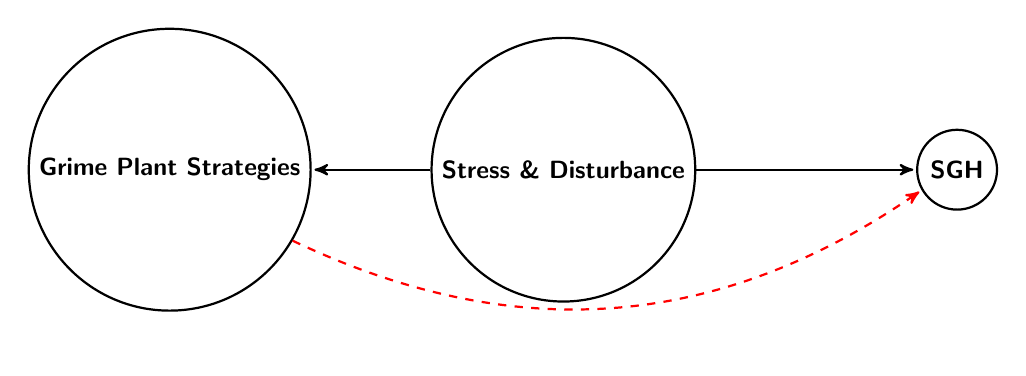
\begin{tikzpicture}[->,>=stealth',shorten >=1pt,auto,node distance=5cm,
                    thick,main node/.style={circle,draw,font=\sffamily\small\bfseries}]

  \node[main node] (1)  {Stress \& Disturbance};
  \node[main node] (2) [right of=1] { SGH };
  \node[main node] (3) [left of=1] {Grime Plant Strategies};

  \path[every node/.style={font=\sffamily\small}]
    (1) edge  node[right] {} (2)
    (1) edge  node {} (3)
    (3) edge [bend right,red, dashed] node  {} (2);
\end{tikzpicture}
\end{center}
\caption{In black: existing links in litterature. In red: Target link to add.}
\end{figure}


The conceptual model of Grime predict the dominant plant strategies along stress and disturbance gradient (Competitive, Stress-tolerator and Ruderals) and SGH predict importance of interaction type along stress and disturbance gradient.

\begin{figure}
\begin{center}
\includegraphics[width=0.5\textwidth]{grime_english.pdf}
\end{center}
\caption{Diagramme of Grime plant strategies along a gradient of Stress and disturbance.\label{Grime}}
\end{figure}



The goal of this studies is to make a conceptual link between Grime and SGH model: (i) Facilitation can modulate Grime predictions ? (ii) Which strategies is the most facilitated along a stress and disturbance gradient ?

\part{Methods}

\section{Site}

The experiment will take in Alicante. Mart's field sites are free to use and those sites seem perfect.

\section{Plants}

To following Grime plant strategies, the best would be to choose species which are enough caricatural. A first axis to separate  quite clear to separate species  difference of ressources management is the SLA (Surface Leaf Area). \textit{To Complete}.
The design would be to plant 3 saplings of 3 different species, each one representing a Grime strategie (See Figure \ref{exp}). An alternative would be to test a set of 2 saplings by treatment: Competitive vs Stress-tolerator for Stress (Water), Competitive vs Ruderals for disturbance gradient (grazing) because we have not hypothesis with for the third sapling.

\begin{figure}
\begin{center}
\includegraphics[width=0.8\textwidth]{Experiment.pdf}
\end{center}
\caption{Représentation graphique de l'expérimentation. Cercle: Adulte; Carré: plantule. Les plantules sont disposées de façon triangulaire sous la nurse, leur disposition étant tirée aléatoirement. \label{exp}}
\end{figure}

Table \ref{hyp} shows assumptions about results of winning strategies according to stress or disturbance. In Summary, (i) we can think facilitation modulate Grime's prediction, (ii) we also make hypothesis that different strategies have different potential to be facilited.



\begin{table}
\begin{center}
\begin{tabular}{|l|l|l|l|l|l|}
  \hline
  & Control & Water stress & Low grazing & High grazing  \\
  \hline
  Patch & C & C & C & R \\
  \hline
  Open & C & S & S ou R & R \\
  \hline
\end{tabular} 
\end{center}
\caption{Hypothesis about winning plant strategies according to stress or disturbance.  Strategies: C (Competitive), R (Ruderal), S (Stress-tolerator). \label{hyp}}
\end{table}



\bibliographystyle{plainnat}

\bibliography{/home/alain.danet/Dropbox/Shared_TheseAlain/BibTeX/M2-StageM2,/home/alain.danet/Dropbox/Shared_TheseAlain/BibTeX/Thesis}
\end{document}
